% !TeX spellcheck = en_EN_english
\documentclass[a4paper]{article}
\usepackage[slovak]{babel}
\usepackage[utf8]{inputenc}
\usepackage[T1]{fontenc}
\usepackage{a4wide}
\usepackage{amsmath}
\usepackage{amsfonts}
\usepackage{amssymb}
\usepackage{mathrsfs}
\usepackage[small,bf]{caption}
\usepackage{subcaption}
\usepackage{xcolor}
\usepackage{graphicx}
\usepackage{enumerate}
\usepackage{hyperref}



\pagestyle{empty}
\setlength{\parindent}{0pt}

\newenvironment{modenumerate}
{\enumerate\setupmodenumerate}
{\endenumerate}

\newif\ifmoditem
\newcommand{\setupmodenumerate}{%
	\global\moditemfalse
	\let\origmakelabel\makelabel
	\def\moditem##1{\global\moditemtrue\def\mesymbol{##1}\item}%
	\def\makelabel##1{%
		\origmakelabel{##1\ifmoditem\rlap{\mesymbol}\fi\enspace}%
		\global\moditemfalse}%
}

\makeatletter
\def\@seccntformat#1{%
	\expandafter\ifx\csname c@#1\endcsname\c@section\else
	\csname the#1\endcsname\quad
	\fi}
\makeatother

\begin{document} 
	
	\pagenumbering{arabic}
	\pagestyle{plain}

	\begin{center}
		\sc\large
		Theoretical homework 2
		
		2-AIN-150, Winter 2023
		
		Theory of ML
	\end{center}
	
	Autor: Marián Kravec
	
	\section{a)}
	
	The hypothesis set $H$ comprises all circles in the plane. Any circle in the plane can be precisely defined by three parameters: two for establishing the center $C=(c_1,c_2)$ of the circle (a 2D point represented by two numbers), and one for determining the radius $r$ of the circle. According to this definition, a point $X=(x_1,x_2)$ is considered inside the circle if it satisfies the inequality $|C-X|\leq r$. Therefore, this hypothesis involves three parameters: two for the center coordinates and one for the radius.
	
	Now we can try to compute $VC$ dimension of this hypothesis set.
	
	Let's start simply and prove that $VC(H) \geq 2$.
	This is simple as if we put two points ($X_1$, $X_2$) in a way that distance between those points will be non-zero:
	
	\centerline{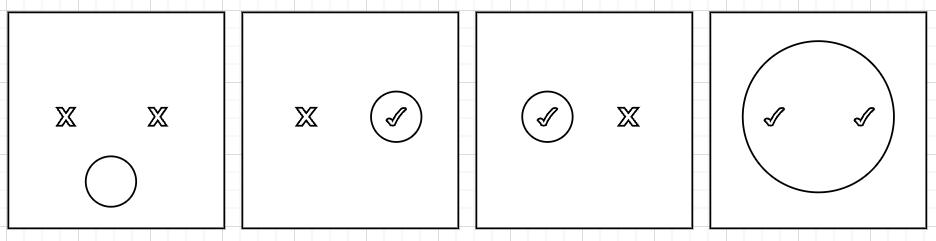
\includegraphics[width=0.9\textwidth]{circles_2}} 
	
	Similarly if we put points into to the triangular shape we can prove that $VC(H) \geq 3$:
	
	\centerline{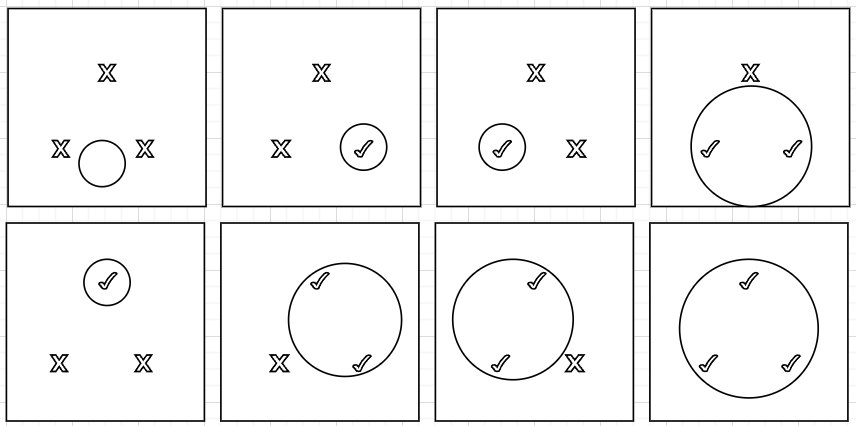
\includegraphics[width=0.9\textwidth]{circles_3}} 
	
	Now we should take a look at $VC(H) ? 4$. Let's analyze it first. If we put two points on each other we can't split them in case they would have opposite classification so all points need to have non-zero distance between each other. Given that our set of hypotheses comprises convex shapes, the placement of three points on a single line presents a challenge. If the central point is negative while the two others on the line are positive, no circle exists that can accurately classify all three points. This restriction implies that at most two points can lie on a single line. Consequently, only two scenarios remain: either three points form a rectangle with the fourth in the middle, or all four points collectively create a convex quadrilateral.
	\\
	\\
	Consider the scenario where a triangle is formed with the fourth point situated in the middle. The issue with this arrangement arises from the convex nature of our hypothesis. If all three points creating the triangle (which is inherently convex) are positive, then all points within the triangle will be classified as positive. Consequently, if the point in the middle is negative, there is no circle that can accurately classify all four points. The challenge lies in the inherent contradiction between the convex nature of the triangle and the attempt to encompass a negative point within it.
	\\
	\\
	Now let's look at case when they create convex quadrilateral.  Any such quadrilateral possesses either four right angles or one obtuse angle. Let's denote our points as $A$, $B$, $C$, and $D$. Without loss of generality, assume that angle $\angle ABC$ is obtuse (or right). In this context, we label points $A$ and $C$ as positive and $B$ as negative, with no consideration for $D$. The smallest circle containing both $A$ and $C$ has a diameter equal to the distance between these points, implying that $A$ and $C$ lie on the circle's edge, and its center lies on the line between them. We can treat this circle as Thale's circle for the segment $AC$, indicating that for any point $X$, if angle $\angle AXC$ is obtuse, the point is inside the circle; if it's right, the point lies on the circle's edge; and if it's acute, the point is outside the circle. Given that angle $\angle ABC$ is obtuse or right, point $B$ is either inside the circle or on its edge. In either case, it will be erroneously labeled as positive, contradicting our initial classification of it as negative. This argument holds for the smallest possible circles, and it extends to any larger circle, as they are merely supersets of the smallest circle.
	\\
	\\
	Now we showed that for any set of four points there exist labeling which can't be split correctly by any of our hypothesis. Now we have proved that $VC(H) < 4$. Which means that  $VC(H) = 3$.

	\section{b)}
	
	This hypothesis set exhibits a notable resemblance to the one described in part a). It can be defined similarly with the utilization of three parameters. Two of these parameters establish the coordinates of the left-bottom corner of a square, denoted as $C=(c_1, c_2)$, and the third parameter represents the length of the side of that square, denoted as $l$. For a point $X=(x_1,x_2$) to be positively classified (i.e., inside the square), it must satisfy the following equations: $c_1 \leq x_1 \leq c_1+l$ and $c_2 \leq x_2 \leq c_2+l$. Now let's try to find out $VC$ dimension of this set.
	
	Let's start simply and prove that $VC(H) \geq 2$.
	This is simple as if we put two points ($X_1$, $X_2$) in a way that distance between those points will be non-zero:
	
	\centerline{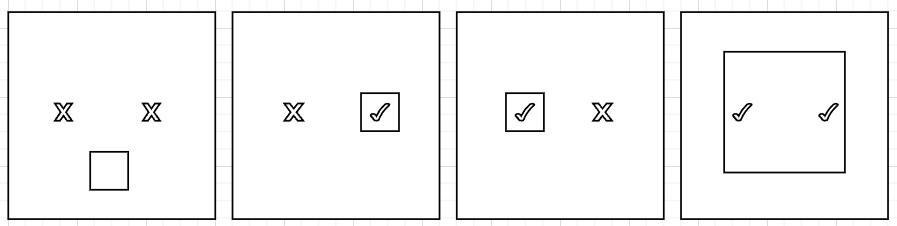
\includegraphics[width=0.9\textwidth]{square_2}} 
	
	Similarly if we put points into to the triangular shape we can prove that $VC(H) \geq 3$:
	
	\centerline{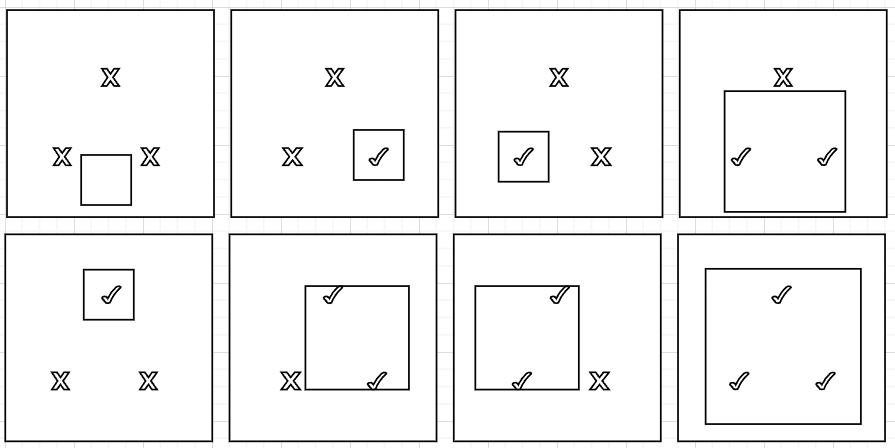
\includegraphics[width=0.9\textwidth]{square_3}} 
	
	Now it's time to take a look at $VC(H) ? 4$. This set is subject to similar constraints as the one in part a).The prohibition of having two points coincide holds, as it would inevitably lead to the same classification for both points, causing issues when they belong to opposing classes. The constraints regarding three points lying on a line remain applicable, given that squares, like circles, are convex shapes. Triangle with forth point in middle is also problem, again because of convex nature of our set and of triangle. That leave only situation when points forms a convex quadrilateral.
	\\
	\\
	Let's split this situation further into sub-situations. In any convex quadrilateral exist leftmost, rightmost, topmost and bottommost point (let's call them "most" points). We will split problem based on how many points we need to choose to have a set containing all four of these points. 
	\\
	\\
	Firstly situation where "most" points set less then 4 points, meaning at least one point is appear two times in "most" point set (e.g. leftmost and topmost). In this case if we label "most" points as positive and rest as negative we get into situation where any square containing "most" points would contain all points because there would always exist point with small and with bigger (or equal) coordinate for both $x_1$ and $x_2$ and if we look at equations point need to satisfy to be labeled positive we can see that our negative point satisfy it and so is incorrectly labeled.
	\\
	\\
	Other situation is that "most" point set contain all points. In this situation each point is exactly one "most" point. Now we will compute two values, $l_1$ which is difference of $x_1$ coordinates of leftmost and rightmost point and $l_2$ which is difference of $x_2$ coordinates of topmost and bottommost point. Now we compare $l_1$ and $l_2$, if $l_1$ is bigger we label leftmost and rightmost as positive and topmost and bottommost as negative, if $l_2$ is bigger we do the opposite. Let's look at the situation where $l_1$ is bigger (other situation is analogous), square that contains both positive points must have side length at least $l_1$ because that's distance between positive points on $x_1$ axis. We know that on $x_2$ axis positive points are between negative (because negative are topmost and bottommost), we know that distance between negative points on $x_2$ is $l_2$ which is smaller than $l_1$ and because of this any square that have side length at least $l_1$ and contain point with $x_2$ value between negative points must necessary contain at least one of negative points and so it will label it incorrectly.
	\\
	\\
	Now we proved that for any set of four points there exist labeling which can't be split correctly by any of our hypothesis. Now we have proved that $VC(H) < 4$. Which means that  $VC(H) = 3$.
	
\end{document}